%%%%%%%%%%%%%%%%%%%%%%%%%%%%%%%%%%%%%%%%%%%%%%%%%%%%%%%%%%%%%%%%%%%%%%%%%%%

\documentclass[a4paper,oneside,12pt]{article}
\usepackage{mystyle}

\begin{document}

\title{\Large\bf Trigonometric functions}
\author{%%
  Minh Van Nguyen \\
  \url{mvngu@gmx.com}
}
\date{\today}
\maketitle

\begin{itemize}
\item Application: equations of parabolic motion for projectiles.
\end{itemize}


%%%%%%%%%%%%%%%%%%%%%%%%%%%%%%%%%%%%%%%%%%%%%%%%%%%%%%%%%%%%%%%%%%%%%%%%%%%

\section{The sine and cosine functions}

By now, you should be familiar with the sine function $\sin x$ and the
cosine function $\cos x$, where $x$ is an angle in radians.  In this
section, you will further investigate properties of the sine and
cosine functions.

\begin{figure}[!htbp]
\centering
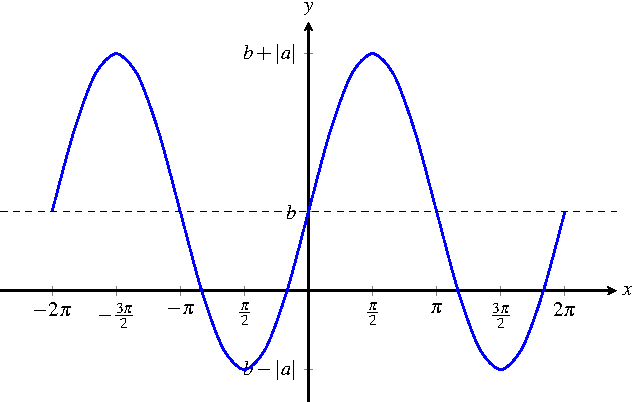
\includegraphics[scale=1.1]{image/13/a-sin-b.pdf}
\caption{%%
  A graph of the general sine function
  $f(x) = a \sin x + b$ from $x = -2\pi$ to $x = 2\pi$.  The midline
  of $f(x)$ is the dashed horizontal line $y = b$.  The amplitude of
  $f(x)$ is the absolute value $\absoluteValue{a}$.
}
\label{fig:trigonometric:general_sine}
\end{figure}

Let $a$ and $b$ be fixed real numbers and let $x$ be a real variable
that represents an angle in radians.  The general sine and cosine
functions can be written as
%%
\begin{equation}
\label{eqn:trigonometric:general_sine_cosine}
f(x)
=
a \sin x + b
%%
\qquad
\text{and}
\qquad
%%
g(x)
=
a \cos x + b.
\end{equation}
%%
In the case of the sine function $f(x) = a \sin x + b$, the number $b$
is called the \emph{midline} of $f(x)$ and the absolute value
$\absoluteValue{a}$ is called the \emph{amplitude} of $f(x)$.
\Figure{fig:trigonometric:general_sine} shows a graph of the general
sine function $f(x)$.  The amplitude $\absoluteValue{a}$ measures how
high and how low the value of the sine function $f(x)$ can be.  As you
can see in \Figure{fig:trigonometric:general_sine}, given the sine
function $f(x) = a \sin x + b$ the highest value of $f(x)$ is
$b + \absoluteValue{a}$ and the lowest value of $f(x)$ is
$b - \absoluteValue{a}$.  The number $b$ is the midline of the sine
function $f(x)$ because the horizontal line $y = b$ is midway between
the highest and lowest values of $f(x)$.  If you draw the horizontal
line $y = b$ on a graph of $f(x)$~(e.g.~the dashed horizontal line in
\Figure{fig:trigonometric:general_sine}) you will see that $f(x) = b$
whenever $a \sin x = 0$.

\end{document}
